\section{Introduction}

Geometry has repeatedly emerged as a powerful organizing principle in physics. General relativity interprets gravitation through the curvature of spacetime, gauge theories describe interactions through connections on fiber bundles, and geometric phases reveal how global properties emerge from local evolution \cite{Einstein1915,Berry1984}. In each case, geometry provides more than a mathematical description; it identifies the fundamental structures governing physical response. A similar development has unfolded across thermodynamics and statistical physics. Over the past several decades, geometric ideas have appeared in equilibrium fluctuation theory, critical phenomena, stochastic thermodynamics, information geometry, synchronization, quantum thermodynamics, and open quantum systems \cite{Weinhold1975,Ruppeiner1979,Ruppeiner1995,Amari2000,Seifert2012}. Yet these developments have largely evolved in parallel, often employing different mathematical languages and emphasizing different physical applications. The extent to which they represent manifestations of a common underlying structure remains an open question.

The central thesis of this review is that the recurring appearance of geometry throughout thermodynamics is not accidental. Rather, geometry emerges because thermodynamics is fundamentally a theory of response. Thermodynamic systems are characterized not only by their states but by how those states respond to perturbations, constraints, environmental interactions, and observations. From this perspective, geometry is not a property of thermodynamic states alone; it is a property of how those states respond. The various geometric structures that appear throughout thermodynamics—metrics, connections, curvature, and holonomy—arise as different manifestations of this underlying response geometry.

The earliest examples of thermodynamic geometry arose in equilibrium statistical mechanics. Building upon Einstein’s theory of fluctuations, Weinhold and Ruppeiner demonstrated that thermodynamic response functions naturally define metric structures on spaces of equilibrium states \cite{Einstein1910,Weinhold1975,Ruppeiner1979,Ruppeiner1995}. These metrics encode susceptibilities, stability, and critical behavior through local notions of distance and curvature. Near critical points, diverging fluctuations induce singular geometric structures whose properties reflect the growth of correlations and the breakdown of characteristic length scales \cite{Ruppeiner1995,Gu2010}. Information geometry provides a closely related perspective in which distinguishability between neighboring probability distributions is quantified through the Fisher information metric and its quantum generalizations \cite{Fisher1925,Amari2000,BraunsteinCaves1994,Paris2009}. Together, these approaches establish a geometric interpretation of fluctuations, stability, and statistical distinguishability.

The geometric character of thermodynamics becomes even more pronounced away from equilibrium. The development of stochastic thermodynamics elevated fluctuating trajectories to fundamental objects and established exact relationships connecting work, entropy production, and irreversibility \cite{Jarzynski1997,Crooks1999,Seifert2012}. Within this framework, geometric phases and pumping phenomena emerge naturally when systems are driven through cyclic variations of control parameters \cite{Sinitsyn2007,Sinitsyn2009}. Excess work, excess entropy production, and nonequilibrium transport acquire geometric interpretations closely analogous to Berry phases in quantum mechanics. These developments suggest that geometry is not merely associated with equilibrium state spaces but is a more general property of thermodynamic response itself.

A complementary line of development concerns synchronization and collective dynamics in driven and dissipative systems. Beginning with the observations of Huygens and extending through the modern theory of coupled oscillators, synchronization provides a paradigmatic example of emergent order arising from interactions among many dynamical degrees of freedom \cite{Kuramoto1984,Strogatz2003}. More recently, synchronization has been extended to quantum systems, where common environments and correlated dissipation can generate phase locking, collective oscillations, and enhanced coherence \cite{Mari2013,Giorgi2013,Bittner2024Sync,Bittner2025JCP}. These studies challenge the traditional view of dissipation as a purely destructive process and instead reveal its capacity to generate organization and collective structure. From a geometric perspective, synchronization may be viewed as the emergence of effective dynamical manifolds and collective coordinates that constrain and organize system response. In this sense, synchronization provides a bridge between nonequilibrium dynamics and response geometry.

Parallel developments in quantum information theory have further expanded the geometric viewpoint. Quantum Fisher information, Bures metrics, and thermodynamic length provide geometric measures of sensitivity, distinguishability, and dissipation in quantum systems \cite{Uhlmann1976,BraunsteinCaves1994,Zanardi2007,Gu2010,Paris2009}. These constructions have become central tools for characterizing quantum phase transitions, parameter estimation, and quantum thermodynamic processes. More generally, they reinforce the idea that response, rather than state alone, provides the natural foundation for geometric descriptions of physical systems.

Open quantum systems provide a particularly rich setting in which these themes converge. Environmental interactions generate decoherence, relaxation, synchronization, collective behavior, and nonequilibrium steady states while simultaneously producing new forms of response unavailable in isolated systems. Recent work has demonstrated that open quantum systems may support geometric structures including work one-forms, curvature two-forms, geometric phases, and holonomies defined on manifolds of control parameters \cite{SivakCrooks2012,NESSGeometry2019,GeometricThermoOQS2026}. At the same time, dissipative phase transitions and Liouvillian criticality reveal striking analogies between nonequilibrium steady states and equilibrium critical phenomena \cite{Prosen2010,DissipativeCriticality2025}. These results suggest that nonequilibrium response possesses a geometric structure that extends, and in some cases transcends, traditional equilibrium formulations.

Taken together, these developments point toward a broader unifying picture. Much of the existing literature has focused on geometric structures associated with states and probability distributions. Metrics derived from thermodynamic potentials, entropy functions, or statistical distinguishability characterize fluctuations, susceptibilities, and stability. Yet nonequilibrium systems reveal an additional geometric sector associated with circulation, transport, and cyclic response. Work performed around thermodynamic cycles, geometric pumping, excess entropy production, and nonequilibrium transport all depend upon path-dependent response rather than state properties alone.

We therefore propose that a complete thermodynamic geometry contains both a symmetric metric sector and an antisymmetric curvature sector. The symmetric sector encodes fluctuations, susceptibilities, stability, and distinguishability. The antisymmetric sector encodes circulation, transport, irreversibility, cyclic work, and geometric phase accumulation. From this perspective, the distinction between fluctuations, transport, work, and information reflects different projections of a common response geometry. Metrics characterize what nearby states can be distinguished; curvature characterizes how response accumulates as systems are transported through parameter space.

The goal of this review is to synthesize these developments and explore the consequences of this viewpoint. We argue that geometry is not a property of thermodynamic states alone but of how those states respond. This perspective provides a common framework linking equilibrium fluctuations, critical phenomena, stochastic thermodynamics, synchronization, information geometry, open quantum systems, and observational descriptions. Throughout, our aim is not merely to survey existing results but to identify the common principles that may underlie a unified geometric theory of thermodynamic response.

\subsection{Historical Development of Thermodynamic Geometry}

The relationship between geometry and thermodynamics has a long and complex history. Although modern discussions often focus on geometric metrics or information-theoretic constructions, many of the underlying ideas can be traced to the earliest formulations of thermodynamics itself. Concepts such as state space, equilibrium manifolds, cyclic processes, and integrability conditions are geometric in character, even when not explicitly expressed in the language of differential geometry.

In classical thermodynamics, the geometric viewpoint emerged naturally through the work of Gibbs and Carathéodory. Equilibrium states were represented as points on thermodynamic manifolds, while thermodynamic processes corresponded to trajectories connecting neighboring states. The existence of thermodynamic potentials and Maxwell relations reflected underlying integrability conditions, and the work performed during cyclic processes was associated with areas enclosed in thermodynamic state spaces. These constructions established a geometric foundation for thermodynamics long before the development of modern thermodynamic geometry.

A more explicit geometric formulation emerged through fluctuation theory. Einstein’s theory of thermodynamic fluctuations revealed a close connection between probability distributions and local response functions, suggesting that fluctuations define a natural notion of distance between neighboring equilibrium states. Building on these ideas, Weinhold introduced a metric structure derived from the Hessian of the internal energy, while Ruppeiner developed an entropy-based metric directly related to fluctuation probabilities. These approaches demonstrated that thermodynamic susceptibilities define local geometric structures whose properties encode stability, correlations, and critical behavior. Over subsequent decades, thermodynamic metrics were applied extensively to fluids, magnetic systems, black-hole thermodynamics, and critical phenomena, establishing metric geometry as one of the central themes of modern thermodynamics.

A second major development arose from information theory and statistical inference. Fisher’s information metric provided a measure of distinguishability between neighboring probability distributions and established a geometric framework for statistical estimation. The subsequent development of information geometry extended these ideas to broad classes of statistical models, while quantum generalizations led to the Bures metric, quantum Fisher information, and related measures of quantum distinguishability. These constructions linked geometry, information, and thermodynamics through a common notion of statistical response, revealing deep connections between fluctuations, inference, and sensitivity to external perturbations.

The scope of thermodynamic geometry expanded dramatically with the development of nonequilibrium statistical mechanics and stochastic thermodynamics. In these frameworks, fluctuating trajectories rather than equilibrium states become the fundamental objects of description. Fluctuation theorems, entropy production, and nonequilibrium work relations revealed new forms of thermodynamic structure that depend explicitly on paths through parameter space. Geometric phases, pumping phenomena, and excess thermodynamic quantities emerged as natural consequences of cyclic driving, introducing geometric concepts closely analogous to Berry phases and gauge fields into nonequilibrium thermodynamics. These developments suggested that thermodynamic geometry extends beyond metrics on state spaces and includes path-dependent structures associated with transport and irreversibility.

At the same time, studies of synchronization and collective dynamics revealed another route by which geometry enters thermodynamics. Classical and quantum synchronization demonstrate how interactions and environmental couplings can generate collective coordinates, reduced manifolds, and emergent dynamical organization. These phenomena suggest that geometry may arise not only from the structure of equilibrium states but also from the mechanisms that organize dynamical response. In this sense, synchronization provides a bridge between nonequilibrium dynamics and geometric descriptions of collective behavior.

More recently, geometric approaches have been developed for open quantum systems and nonequilibrium steady states. Dissipative phase transitions, Liouvillian criticality, geometric pumping, and steady-state response have revealed structures involving connections, curvature, and holonomy that have no direct equilibrium analog. These developments indicate that the geometric description of thermodynamics must ultimately encompass both equilibrium and nonequilibrium phenomena, as well as both classical and quantum systems.

Viewed from this historical perspective, thermodynamic geometry has evolved through a sequence of increasingly general frameworks. The earliest formulations emphasized state spaces and integrability. Fluctuation theory introduced metric structures associated with response and stability. Information geometry generalized these ideas to statistical distinguishability. Nonequilibrium thermodynamics introduced path-dependent geometric phases and transport phenomena. Synchronization and collective dynamics revealed the emergence of geometric organization through dissipation. Open quantum systems extended these concepts to steady-state manifolds exhibiting curvature and holonomy.

The central theme emerging from this progression is that geometry appears whenever thermodynamic response is examined at a sufficiently fundamental level. The historical development of thermodynamic geometry may therefore be viewed not as a succession of unrelated constructions but as a gradual expansion of the notion of response itself—from equilibrium states, to fluctuations, to trajectories, to collective dynamics, and ultimately to observable-dependent descriptions. This broader perspective motivates the central thesis of the present review: geometry is not a property of thermodynamic states alone but of how those states respond.


\begin{figure*}[t]
\centering
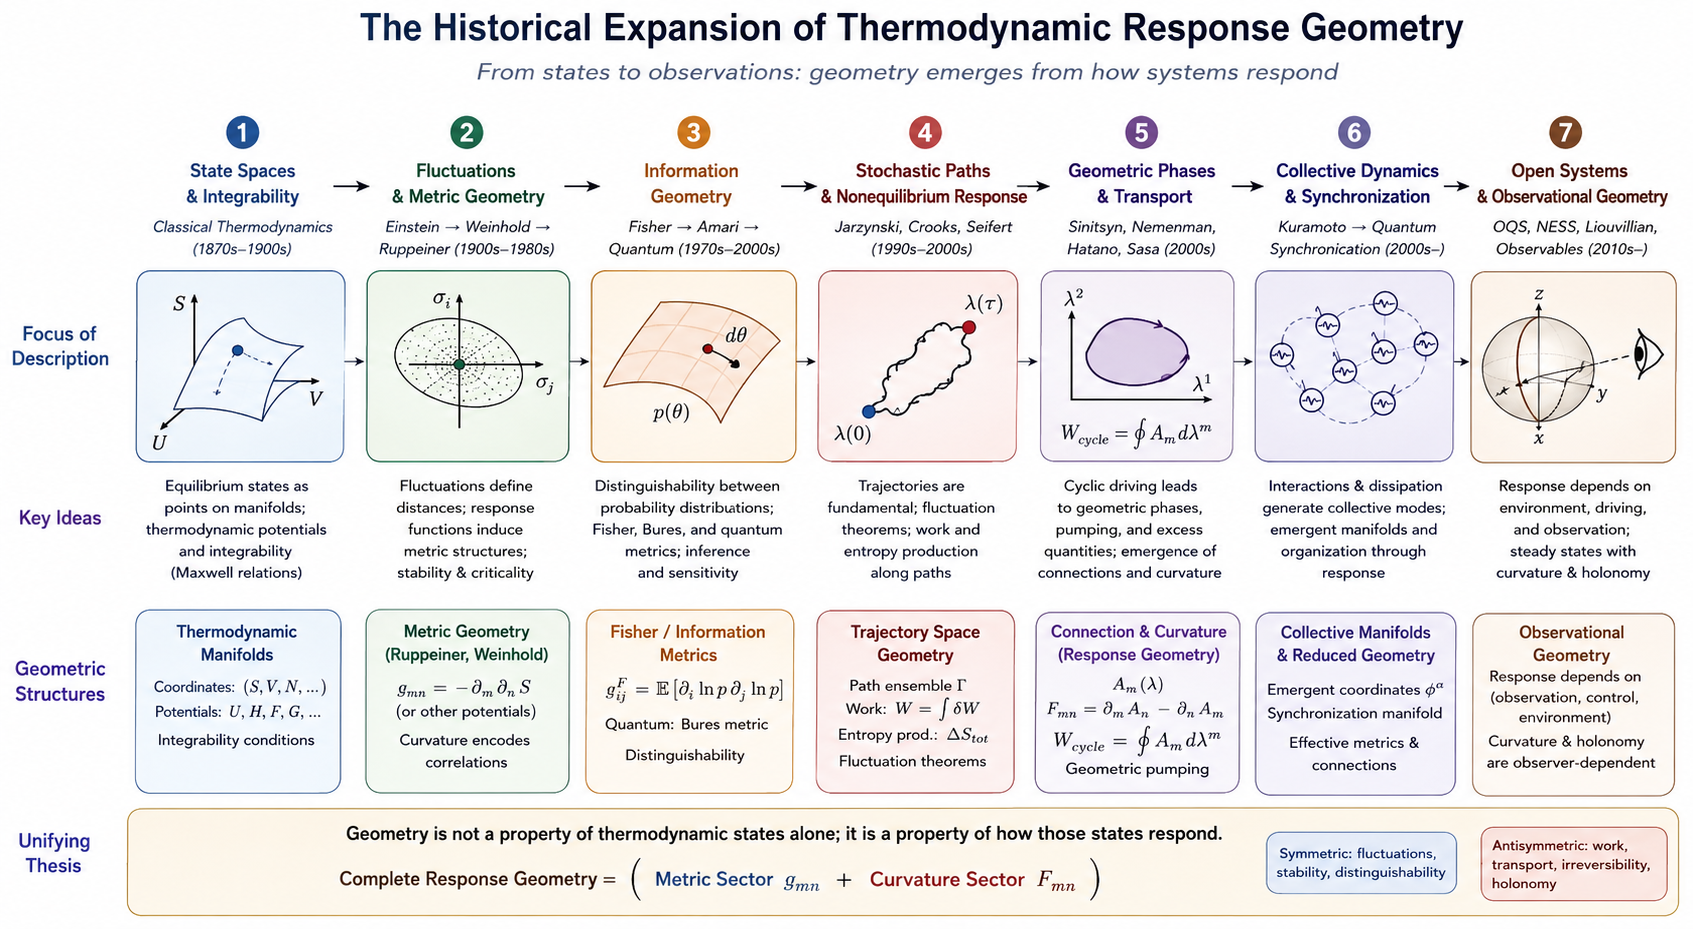
\includegraphics[width=\textwidth]{Figures/2F7A6768-CD89-4332-9FC2-827ED817DBA7.png}
\caption{
Conceptual progression of the response-geometry program.
(\textbf{a}) Classical thermodynamics, where response is encoded by
equilibrium fluctuations and susceptibilities, giving rise to
geometric structures such as metrics, curvature, and cycle
holonomies on the thermodynamic state manifold.
(\textbf{b}) Open quantum systems, where environmental interactions
generate nonequilibrium steady states and induce geometric
response through coherence, dissipation, and basis
misalignment between energy and pointer representations.
(\textbf{c}) Observable-conditioned thermodynamics, in which the
geometry depends explicitly on the observational frame,
leading to gauge-like structures associated with restricted
access to system information.
(\textbf{d}) Spectroscopic reconstruction, where geometric quantities
are inferred from experimentally accessible observables,
including nonlinear optical response, intensity borrowing,
and bright–dark state mixing. In this picture, curvature,
connections, and holonomy emerge as measurable properties
of response rather than purely abstract mathematical
constructions. The overall program seeks to establish a
unified geometric description of thermodynamic response
across equilibrium, nonequilibrium, and quantum regimes.
}
\label{fig:program_cartoon}
\end{figure*}


\section{Metrics, Connections, Curvature, and Response}

Geometric descriptions of physical systems generally arise
from four closely related structures: a metric, a connection,
a curvature, and the corresponding response functions that
render these quantities observable. Although these objects
appear in diverse contexts ranging from general relativity
to gauge theory and information geometry, they share a
common interpretation as measures of how a system changes
under variation of external parameters.

The most familiar geometric object is the metric tensor.
A metric defines a local notion of distance on a manifold and
thereby quantifies distinguishability between neighboring
states. In thermodynamics, the Weinhold and Ruppeiner
metrics relate this notion of distance to susceptibilities and
equilibrium fluctuations. In quantum mechanics, analogous
structures arise through the quantum geometric tensor,
Bures metric, and quantum Fisher information, which
measure the sensitivity of quantum states to parameter
variation. In each case, the metric characterizes the local
response of the system and provides a geometric measure of
its fluctuations.

A metric alone, however, does not determine how local
information is compared across different points of a manifold.
This role is played by a connection. A connection specifies
how vectors, operators, or states are transported between
neighboring points and therefore encodes the choice of local
reference frame. Familiar examples include the Levi-Civita
connection of differential geometry, Berry connections in
quantum mechanics, and gauge connections in field theory.
Physically, connections determine how response measured at
one point is related to response measured at another.

Curvature quantifies the extent to which parallel transport
depends on path. Equivalently, it measures the failure of
successive parameter variations to commute. In differential
geometry, curvature governs the holonomy acquired by a
vector transported around a closed loop. In gauge theories,
it corresponds to the field strength tensor. In quantum
mechanics, Berry curvature determines geometric phases
accumulated under cyclic evolution. More generally,
curvature provides a local measure of nonintegrability:
whenever response depends on the order in which control
parameters are varied, a nonzero curvature is present.

The geometric structures introduced above become physically
meaningful only through response. Metrics are inferred from
fluctuations and susceptibilities, connections from the
transport of local reference frames, and curvature from
cyclic response and holonomy. From this perspective,
geometry is not an abstract property imposed upon a
physical system but rather an emergent description of how
the system responds to external perturbations.

The central premise of the present work is that response
itself may be regarded as a geometric object. Observable
changes induced by parameter variation define local frames
on a control manifold, while the incompatibility of distinct
response channels generates connections and curvature.
This viewpoint naturally unifies equilibrium fluctuation
geometry, nonequilibrium thermodynamic response, and
the geometric structures that arise in open quantum
systems.

\subsection{Scope and Organization of This Review}

The literature connecting geometry and thermodynamics has grown rapidly over the past several decades and now spans diverse areas including equilibrium fluctuation theory, information geometry, stochastic thermodynamics, quantum thermodynamics, nonequilibrium statistical mechanics, synchronization, and open quantum systems. A comprehensive review of all geometric approaches is therefore beyond the scope of a single article. Instead, our objective is to identify the common principles that underlie these developments and to examine them through the unifying concept of response geometry.

Our emphasis is consequently not on providing an exhaustive catalog of geometric constructions, but rather on understanding why geometric structures repeatedly emerge in thermodynamic descriptions. Throughout the review, we focus on the relationship between physical response and geometry, emphasizing how fluctuations, susceptibilities, transport coefficients, entropy production, synchronization, and work may all be interpreted as manifestations of a common geometric framework. Particular attention is devoted to the distinction between metric structures associated with fluctuations and distinguishability, and curvature structures associated with circulation, transport, and cyclic response.

The perspective adopted here naturally spans both classical and quantum systems. We begin with equilibrium thermodynamics, where geometric concepts arise through fluctuations, susceptibilities, and critical phenomena. We then consider stochastic thermodynamics and nonequilibrium response, where geometric phases and excess thermodynamic quantities emerge from trajectory-dependent dynamics. Synchronization and collective behavior are subsequently discussed as examples of geometric organization induced by interactions and dissipation. We then turn to information geometry and open quantum systems, where notions of distinguishability, coherence, and steady-state response reveal increasingly rich geometric structures.

The final sections explore recent developments in observable-dependent thermodynamics and observational geometry. These approaches suggest that geometric structure may depend not only on the underlying dynamics but also on the observational framework through which a system is described. Such ideas point toward a broader conception of thermodynamic geometry in which states, trajectories, controls, environments, and observations all contribute to the geometric characterization of response.

A recurring theme throughout this review is that a complete geometric description of thermodynamics requires both a symmetric and an antisymmetric sector. The symmetric sector, represented by metric structures, characterizes fluctuations, susceptibilities, stability, and distinguishability. The antisymmetric sector, represented by connections and curvature, characterizes circulation, transport, irreversibility, and work. While these structures often appear under different names in different communities, we argue that they are most naturally understood as complementary components of a unified response geometry.


